\documentclass[12pt]{article}
\usepackage{graphicx}
\usepackage{amsmath}
\title{Assignment 1}
\author{Divyansh Wangnue}
\date{\today}


\begin{document}
\maketitle
\pagenumbering{gobble}
\newpage
\pagenumbering{arabic}
\section{ODEMC Lesson Plan}
\subsection{Unit 1}
\paragraph{A first-order differential equation is defined by an equation:(x,y) of two variables x and y with its function f(x,y) defined on a region in the xy-plane. It has only the first derivative dy/dx so that the equation is of the first order and no higher-order derivatives exist}
1. Review of first order differential equations\\
2. Reduction of order\\
3.Linear Differential Equations\\
\subsection{Unit 2}
\paragraph{Laplace transform is the integral transform of the given derivative function with real variable t to convert into a complex function with variable s. For  let f(t) be given and assume the function satisfies certain conditions to be stated later on.}
1. Laplace Transform\\
2. Properties\\
3. Unit step function\\
\subsection{Unit 3}
\paragraph{A function of variables, also called a function of several variables, with domain is a relation that assigns to every ordered -tuple in a unique real number in . We denote this by each of the following types of notation. The range of is the set of all outputs of . It is a subset of , not .}
1. Functions of several variables \\
2. Level curves and level surfaces\\
3. Partial and directional derivatives\\

\newpage
\section{Assignment 2 - Mathematical equations}
\begin{flushleft}
Q.1) Solve the following:\\[10pt]
(a)$3x(xy-2)dx+(x^3+2y)dy=0$\hspace{5.5cm}[CO 2] [2]\\[6 pt]
(b)$(2\cos{y} + 4x^2)dx -x\sin{y}dy==0$\hspace{4.65cm}[CO 2]    [3]\\
\end{flushleft} 



\begin{flushleft}
 Q.2) Find a homogeneous linear second order ordinary differential equation whose solution is the set of all straight lines in the $xy$-plane.\hspace{1cm}[CO 1] [1]\\ 
\end{flushleft}

\begin{flushleft}
 Q.3)State whether the following differential equations are linear or non linear ,justify and solve:\\[10pt]
(a)$xy'+2y = \frac{e^{3x}}{x}, x>0 with y(1)=1+\frac{e^3}{3}. $\hspace{3.5cm}[CO 2] [3]\\[6 pt]
(b)$x^2y\frac{dy}{dx}- xy^2 = 1$\hspace{7.05cm}[CO 2] [3]
\end{flushleft}

\begin{flushleft}
Q.4) If $x^2$ and $1$ are solutions of $yy''-xy'=0$ then so is any linear combination of these. State true or false and justify.\hspace{2cm}[CO 4] [2]
\end{flushleft}

\begin{flushleft}
Q.5) Find a linear ordinary differential equation for which the function $e^{-x}\cos{2x}$ and $e^{-x}\sin{2x}$ are linearly independent solutions.\hspace{0.7cm}[CO 2] [3]
\end{flushleft}


Q.6) Make a matrix
$\begin{bmatrix}
1 & 2 & 3 \\
a & b & c
\end{bmatrix}$



\newpage

\section{Inserting Images}
     \begin{figure} [h]
     \centering
     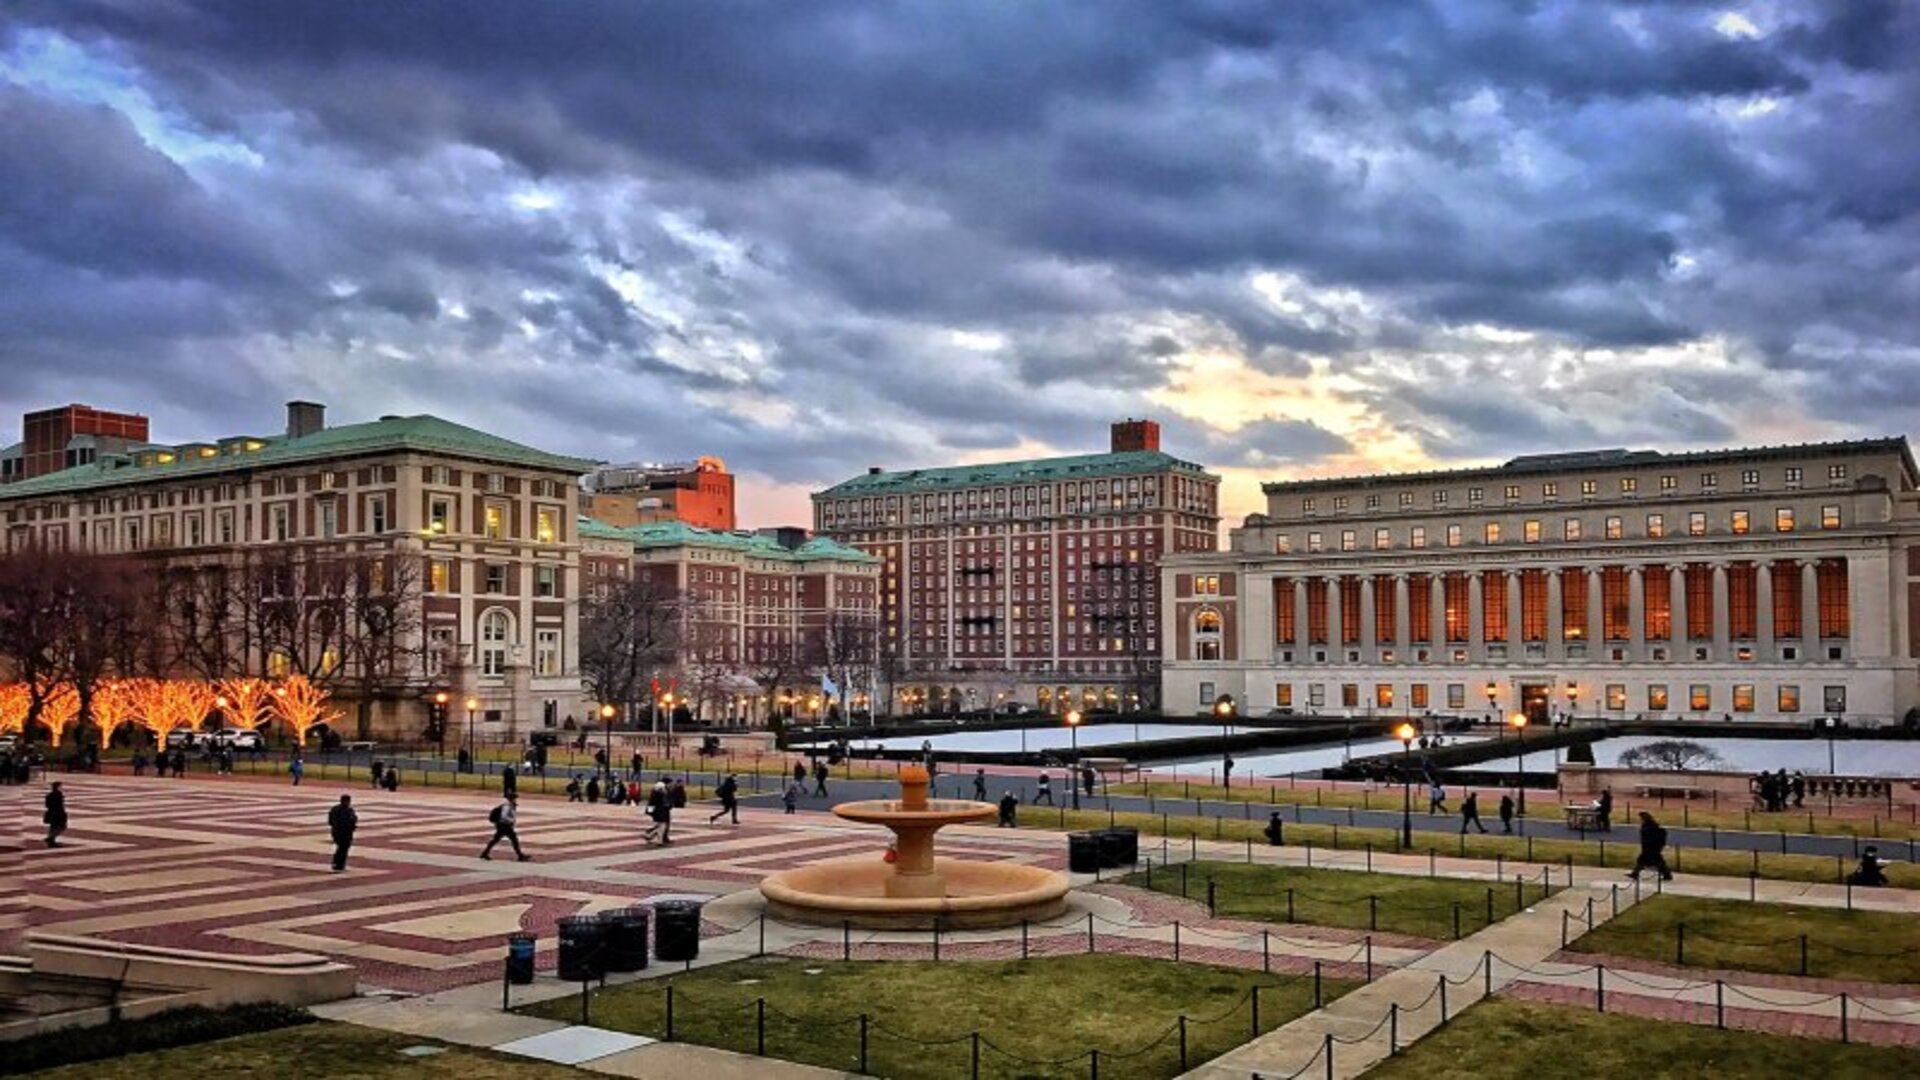
\includegraphics[width=0.8\linewidth]{85.jpg}
     \caption{figure}
      \label{fig:85}
\end{figure}
\newpage





\begin{table}

\section{Tables using latex}

\begin{center}



\caption{Price of various fruits}

\label{ A ) }


\begin{tabular}{|l|c|r|}

\textbf{Sr. no.} & 
\textbf{Fruits} &
\textbf{Price}\\

\hline
1	 & 		Apple		 & 	20		\\
2	 & 		Orange		 & 	40		\\
3	 & 		Guava    	 & 	50		\\
4	 & 		Banana   	 & 	60		\\
5	 & 		Pineapple	 & 	10		\\


\end{tabular}

\end{center}

\end{table}

\end{document}